\usetikzlibrary{arrows.meta}

\begin{figure}[htb]
	\begin{center}
		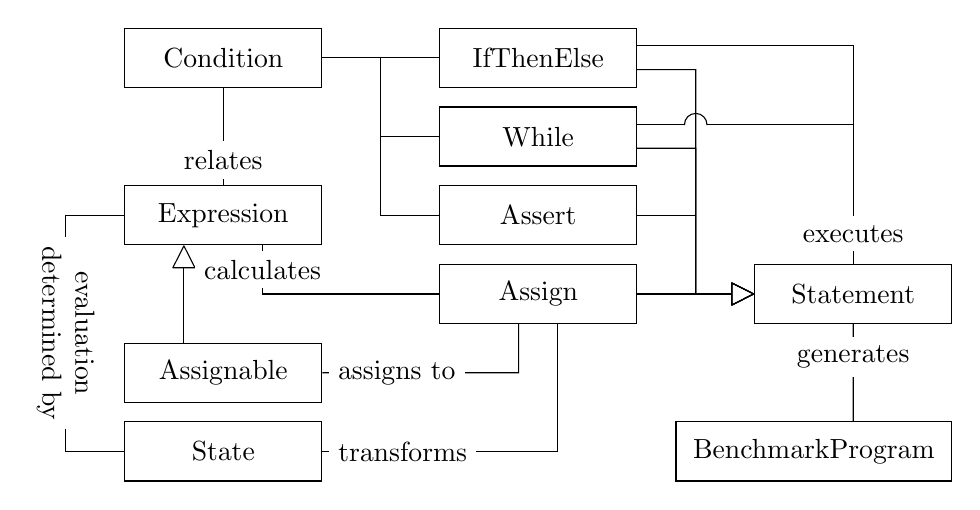
\begin{tikzpicture}
         
 
         \node [rectangle, draw, minimum width=2.5cm, minimum height=0.75cm] (state)       at (0,0)    {State};
         \node [rectangle, draw, minimum width=2.5cm, minimum height=0.75cm] (assignable)  at (0,1)    {Assignable};
         \node [rectangle, draw, minimum width=2.5cm, minimum height=0.75cm] (expression)  at (0,3)    {Expression};
         \node [rectangle, draw, minimum width=2.5cm, minimum height=0.75cm] (condition)   at (0,5)    {Condition};
         
         \node [rectangle, draw, minimum width=2.5cm, minimum height=0.75cm] (ifthenelse)  at (4,5)    {IfThenElse};
         \node [rectangle, draw, minimum width=2.5cm, minimum height=0.75cm] (while)       at (4,4)    {While};
         \node [rectangle, draw, minimum width=2.5cm, minimum height=0.75cm] (assert)      at (4,3)    {Assert};
         \node [rectangle, draw, minimum width=2.5cm, minimum height=0.75cm] (assign)      at (4,2)    {Assign};
         
         \node [rectangle, draw, minimum width=2.5cm, minimum height=0.75cm] (statement)   at (8,2)    {Statement};
         
         \node [rectangle, draw, minimum width=3.5cm, minimum height=0.75cm] (benchmarkprogram) at (7.5,0) {BenchmarkProgram};
         
  		 \draw (state) -- (-2,0) -- node[fill=white!5, align=center, rotate=270]{evaluation\\ determined by} (-2,3) -- (expression);
  		 
  		 \draw (condition) -- node[fill=white!5, yshift=-3mm]{relates} (expression);
  		 \draw ([xshift=-2.5mm]assign.south) -- (3.75,1) -- node[fill=white!5, xshift=-3mm]{assigns to} (assignable);
  		 
  		 \draw [-{Triangle[round,open, length=3mm, width=3mm]}]([xshift=-0.5cm]assignable.north) -- ([xshift=-0.5cm]expression.south);
  		 
  		 \draw (assign) -- (0.5,2) -- node[fill=white!5]{calculates} ([xshift=0.5cm]expression.south);
  		 
  		 
  		 \draw [-{Triangle[round,open, length=3mm, width=3mm]}](assign) -- (statement);
  		 \draw [-{Triangle[round,open, length=3mm, width=3mm]}](assert) -- (6,3) -- (6,2) -- (statement);
  		 \draw [-{Triangle[round,open, length=3mm, width=3mm]}]([yshift=-0.15cm]while.east) -- (6,3.85) -- (6,2) -- (statement);
  		 \draw [-{Triangle[round,open, length=3mm, width=3mm]}]([yshift=-0.15cm]ifthenelse.east) -- (6,4.85) -- (6,2) -- (statement);
		 \draw ([yshift=0.15cm]ifthenelse.east) -- (8,5.15) -- (statement);
         
         

		\draw[-{Arc Barb[harpoon,reversed, length=1.5mm, width=3mm]}] ([yshift=0.15cm]while.east) -- (6,4.15);
		\draw[{Arc Barb[harpoon,reversed,right, length=1.5mm, width=3mm]}-] (6,4.15) -- (8,4.15);
		\draw (8,4.15) -- node[fill=white!5, yshift=-5mm]{executes} (statement);
		
		\draw (assert) -- (2,3) -- (2,5);
		\draw (while) -- (2,4) -- (2,5);
		\draw (ifthenelse) -- (condition);
		
		\draw ([xshift=0.5cm]benchmarkprogram.north) -- node[fill=white!5, yshift=2mm]{generates} (statement);
        
        \draw ([xshift=2.5mm]assign.south) -- (4.25,0) -- node[fill=white!5, xshift=-4.75mm]{transforms} (state);
        
        \end{tikzpicture}
        \caption{A simplified UML-like diagram showcasing the architecture of the implemented analyser.}\label{fig:uml_analyser}
	\end{center}
\end{figure}